\section{Model, graph parameters, and output contracts}
\label{sec:main-model}

Let $G=(V,E)$ be a finite connected loopless graph with a chosen edge
orientation. Parallel edges are permitted except in the universal graph
characterizations, where graphs are simple. Its incidence matrix $A$
has $+1$ at each tail and $-1$ at each head. A balanced nomination
$b\in\R^V$, $\one^\top b=0$, specifies injections and withdrawals.
The signed flow $x$ and potential $\pi$ satisfy
\begin{equation}
 Ax=b,\qquad A^\top\pi=g(x).
 \label{eq:main-state}
\end{equation}
A general passive law $g_e$ is continuous, strictly increasing, and
vanishes at zero. The flow is unique and the potentials are unique up
to an additive constant: the primitives
$F_e(t)=\int_0^t g_e(u)\,du$ are strictly convex and coercive, so
$\sum_e F_e(x_e)$ has a unique minimizer on $Ax=b$, and stationarity
says $g(x)\in\operatorname{im}A^\top$. \Cref{thm:a-pre-existence}
gives the full argument, including bounded laws and the one-vertex case.

Unless stated otherwise, algorithmic results use symmetric quadratic
laws $g_e(t)=\beta_e t|t|$, with positive coefficients. A directional
quadratic law instead uses $\beta_e^+t^2$ for $t\ge0$ and
$-\beta_e^-t^2$ for $t\le0$. Reversing an edge swaps its two
coefficients. An output state has one potential grounded to zero.
Every nonzero physical flow points down a strictly decreasing potential,
so there is no directed circulation, and a source-to-sink path
decomposition bounds $|x_e|$ by the total positive nomination. This
bound is the uniform compactness estimate behind the perturbation and
rounding arguments.

\subsection{Scenario domains}

A balanced nomination box is
\begin{equation}
 \mathcal B=\{b\in\R^V:\ell\le b\le u,\ \one^\top b=0\},
 \qquad \ell,u\in\Q^V,\quad \ell\le u.
 \label{eq:main-box}
\end{equation}
It is nonempty exactly when $\sum_v\ell_v\le0\le\sum_vu_v$.
Shifted intervals, sign-changing nominations, and singleton intervals
are allowed. Another input is an affine balanced family
$b(z)=b^0+Mz$ on a nonempty compact rational polytope
$P\subseteq\R^d$, supplied by linear inequalities and equalities.
Fixed dimension means that $d$ is independent of graph size.

Independent resistance uncertainty means
$\mathcal R=\prod_e[L_e,U_e]$, with rational $0<L_e\le U_e$.
Finite uncertainty means a product of explicitly listed nonempty finite
subsets of $\Q_{>0}$. A global polytope may couple coefficients from
different edges and blocks. A cycle-local polytope couples any number
of law parameters within one cycle, while different cycle polytopes are
independent; the attainable regions of these two models can differ
even on two cycles. Directional and symmetric intervals are also
distinct models: directional intervals are independent positive
intervals for $\beta_e^+$ and $\beta_e^-$, whereas a symmetric interval
constrains one common coefficient for both directions.

A scenario is an admissible original parameter vector, such as
$(b,\beta)$; its state is determined by \eqref{eq:main-state}. Most
nomination theorems use the full \emph{unfiltered} scenario domain.
Robust capacity validation asks whether the arc flow of every such
state satisfies given signed bounds. Capacity \emph{feasibility} and
constrained design instead ask whether some scenario satisfies the
bounds, and optimize only over those scenarios. Such a filter changes
the parameter domain and can remove all rational points even for
rational input. Where filters are allowed, the theorem states their
form and the resulting output type.

\subsection{Observables and precision}

We study a prescribed terminal difference $F_{s,t}=\pi_s-\pi_t$,
a weighted potential $W=c^\top\pi$ with $c\in\Q^V$ and $\one^\top c=0$,
an individual arc flow $x_a$, and a linear flow objective $d^\top x$.
Since $\one^\top c=0$, $W$ does not depend on the gauge; let
$p=|\supp c|$. Maximum potential difference (MPD) means maximizing
$F_{s,t}$ for specified ordered terminals, not a search over terminal
pairs.

For a maximization objective $F$, write
$\OPT=\max_{\theta\in\Theta}F(\theta)$.
An exact threshold question is $\OPT\ge\gamma$ for rational $\gamma$;
equality belongs to the yes case. The additive contract, for rational
$\eps>0$, is
\begin{equation}
 \underline v\le\OPT\le\overline v,\quad
 \overline v-\underline v\le\eps,\quad
 \widehat\theta\in\Theta\cap\Q^k,\quad
 F(\widehat\theta)\ge\OPT-\eps.
 \label{eq:main-contract}
\end{equation}
The output interval is rational and the parameter scenario is exactly
admissible; minimization reverses the inequality. Theorems that promise
only a parameter or an exact algebraic value say so. Algebraic values
are encoded by an integer polynomial and an isolating interval, or an
equivalent real univariate representation. A list of local algebraic
values is an expression for their sum, not necessarily a
polynomial-size algebraic encoding of that sum.

All complexity bounds use the Turing model. Let $N$ denote total binary
input length, including rational tolerances, and put
$N_\eps=N+\max\{0,\lceil\log_2(1/\eps)\rceil\}+1$.
An accuracy-bit polynomial algorithm is polynomial in $N_\eps$, so
each additional bit of accuracy costs only polynomially more; an
algorithm polynomial in $1/\eps$ need not have this property.
A parameter-dependent exponent, such as $N_\eps^{O(r)}$, gives a
polynomial for each fixed $r$; this is an XP-type bound, not
fixed-parameter tractability, which would require $f(r)N_\eps^C$ with
an absolute exponent $C$.

An additive interval decides a threshold when it lies on one side of
it, but repeated refinement alone does not settle equality. Moreover,
rational scenarios need not have rational states. For two unloaded
parallel branches of total resistances $1$ and $2$, a unit transfer
splits as $\sqrt2/(1+\sqrt2)$ and $1/(1+\sqrt2)$, with common drop
$2/(1+\sqrt2)^2$. All inputs are rational, while the flow and drop
are irrational. Rational approximate states therefore need error
bounds; in general they cannot satisfy both physical equations exactly.

\subsection{Block rank and block decomposition}

A block is a biconnected component, with bridges treated as two-vertex
blocks. Write $r_B=|E(B)|-|V(B)|+1$,
$r_{\max}=\max_B r_B$, and
$r=|E|-|V|+1=\sum_B r_B$.
The maximum over no blocks is defined to be zero.
(\Cref{sec:a-pre-preliminaries,sec:a-block-rank,sec:a-laws} write $H$
and $r_H$ for a block and its rank, and $\mathfrak r$ for the bound
written $r_0$ here; \cref{sec:a-weighted-cactus,sec:a-weighted-blocks}
write $H$ for the nomination matrix $M$.) A tree has $r_{\max}=0$; a cactus,
in which distinct simple cycles share at most one vertex (equivalently,
each edge lies on at most one simple cycle), has $r_{\max}\le1$. A chain of $k$ triangles has
$r_{\max}=1$ and $r=k$. Series-parallel means having no $K_4$ minor;
we use this graph property rather than requiring specified decomposition
terminals. A series-parallel block can have arbitrarily large rank:
$K_{2,k}$ has rank $k-1$ and treewidth two.

\begin{figure}[tb]
\centering
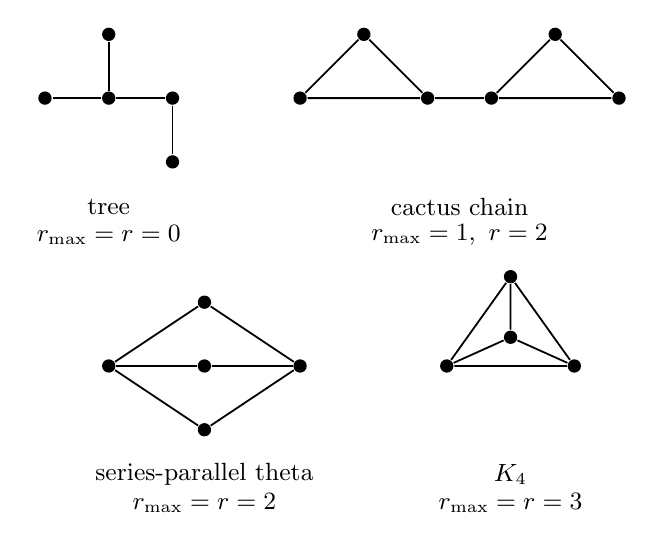
\begin{tikzpicture}[scale=.81, every node/.style={font=\small},
 vertex/.style={circle,fill,inner sep=1.7pt},line width=.65pt]
\begin{scope}
\foreach \n/\x/\y in {a/0/0,b/1/0,c/2/0,d/1/1,e/2/-1}
 \node[vertex] (\n) at (\x,\y) {};
\draw (a)--(b)--(c)--(e) (b)--(d);
\node at (1,-1.7) {tree};
\node at (1,-2.15) {$r_{\max}=r=0$};
\end{scope}
\begin{scope}[xshift=4cm]
\foreach \n/\x/\y in {a/0/0,b/1/1,c/2/0,d/3/0,e/4/1,f/5/0}
 \node[vertex] (\n) at (\x,\y) {};
\draw (a)--(b)--(c)--(a) (c)--(d) (d)--(e)--(f)--(d);
\node at (2.5,-1.7) {cactus chain};
\node at (2.5,-2.15) {$r_{\max}=1,\ r=2$};
\end{scope}
\begin{scope}[xshift=1cm,yshift=-4.2cm]
\node[vertex] (s) at (0,0) {};
\node[vertex] (t) at (3,0) {};
\foreach \i/\y in {1/-1,2/0,3/1}{
 \node[vertex] (v\i) at (1.5,\y) {};
 \draw (s)--(v\i)--(t);}
\node at (1.5,-1.7) {series-parallel theta};
\node at (1.5,-2.15) {$r_{\max}=r=2$};
\end{scope}
\begin{scope}[xshift=6.3cm,yshift=-4.2cm]
\foreach \n/\x/\y in {a/0/0,b/2/0,c/1/1.4,d/1/.45}
 \node[vertex] (\n) at (\x,\y) {};
\draw (a)--(b)--(c)--(a) (d)--(a) (d)--(b) (d)--(c);
\node at (1,-1.7) {$K_4$};
\node at (1,-2.15) {$r_{\max}=r=3$};
\end{scope}
\end{tikzpicture}
\caption{Four graph structures used in the complexity boundaries.
Adding cactus blocks raises total rank without raising maximum block
rank. Adding parallel paths inside one block raises both. The displayed
$K_4$ is the obstruction to universal individual-arc hull equality.}
\label{fig:main-topologies}
\end{figure}

Deleting a block's edges leaves components attached at its vertices.
Summing their nominations gives the block's effective nomination, and
the block's state depends only on that aggregate and its own laws.
Since the block--vertex incidence graph is a tree, a terminal difference
is the sum of drops along its unique block path, while an individual
arc belongs to one block. \Cref{lem:a-pre-block,lem:a-pre-incidence}
prove these facts without assumptions on flow signs. They are why
pressure and arc objectives have different exact-output guarantees.
